\documentclass[twocolumn,letterpaper]{scrartcl}

\usepackage[english]{babel}
\usepackage{blindtext}
\usepackage[margin=1in]{geometry}
\usepackage[sorting=none, maxbibnames=99]{biblatex}
\usepackage[breaklinks=true, colorlinks=True, allcolors=blue]{hyperref}
\usepackage{graphicx}
\usepackage[font={small}]{caption}

\addbibresource{CRB.bib}  


% The following lines add color to title, section, and subsection headings.
% Matches color used for FIDLs.
\usepackage{xcolor}
\definecolor{FIDL}{RGB}{31,98,66}
\addtokomafont{title}{\color{FIDL}}
\addtokomafont{section}{\color{FIDL}}
\addtokomafont{subsection}{\color{FIDL}}

\begin{document}

\titlehead{Forest Insect \& Disease Leaflet}	
\title{Coconut Rhinoceros Beetle}
\author{Aubrey Moore}
\maketitle

%\tableofcontents

%\tableofcontents{}
\newpage

\begin{figure}[h]
	\centering
	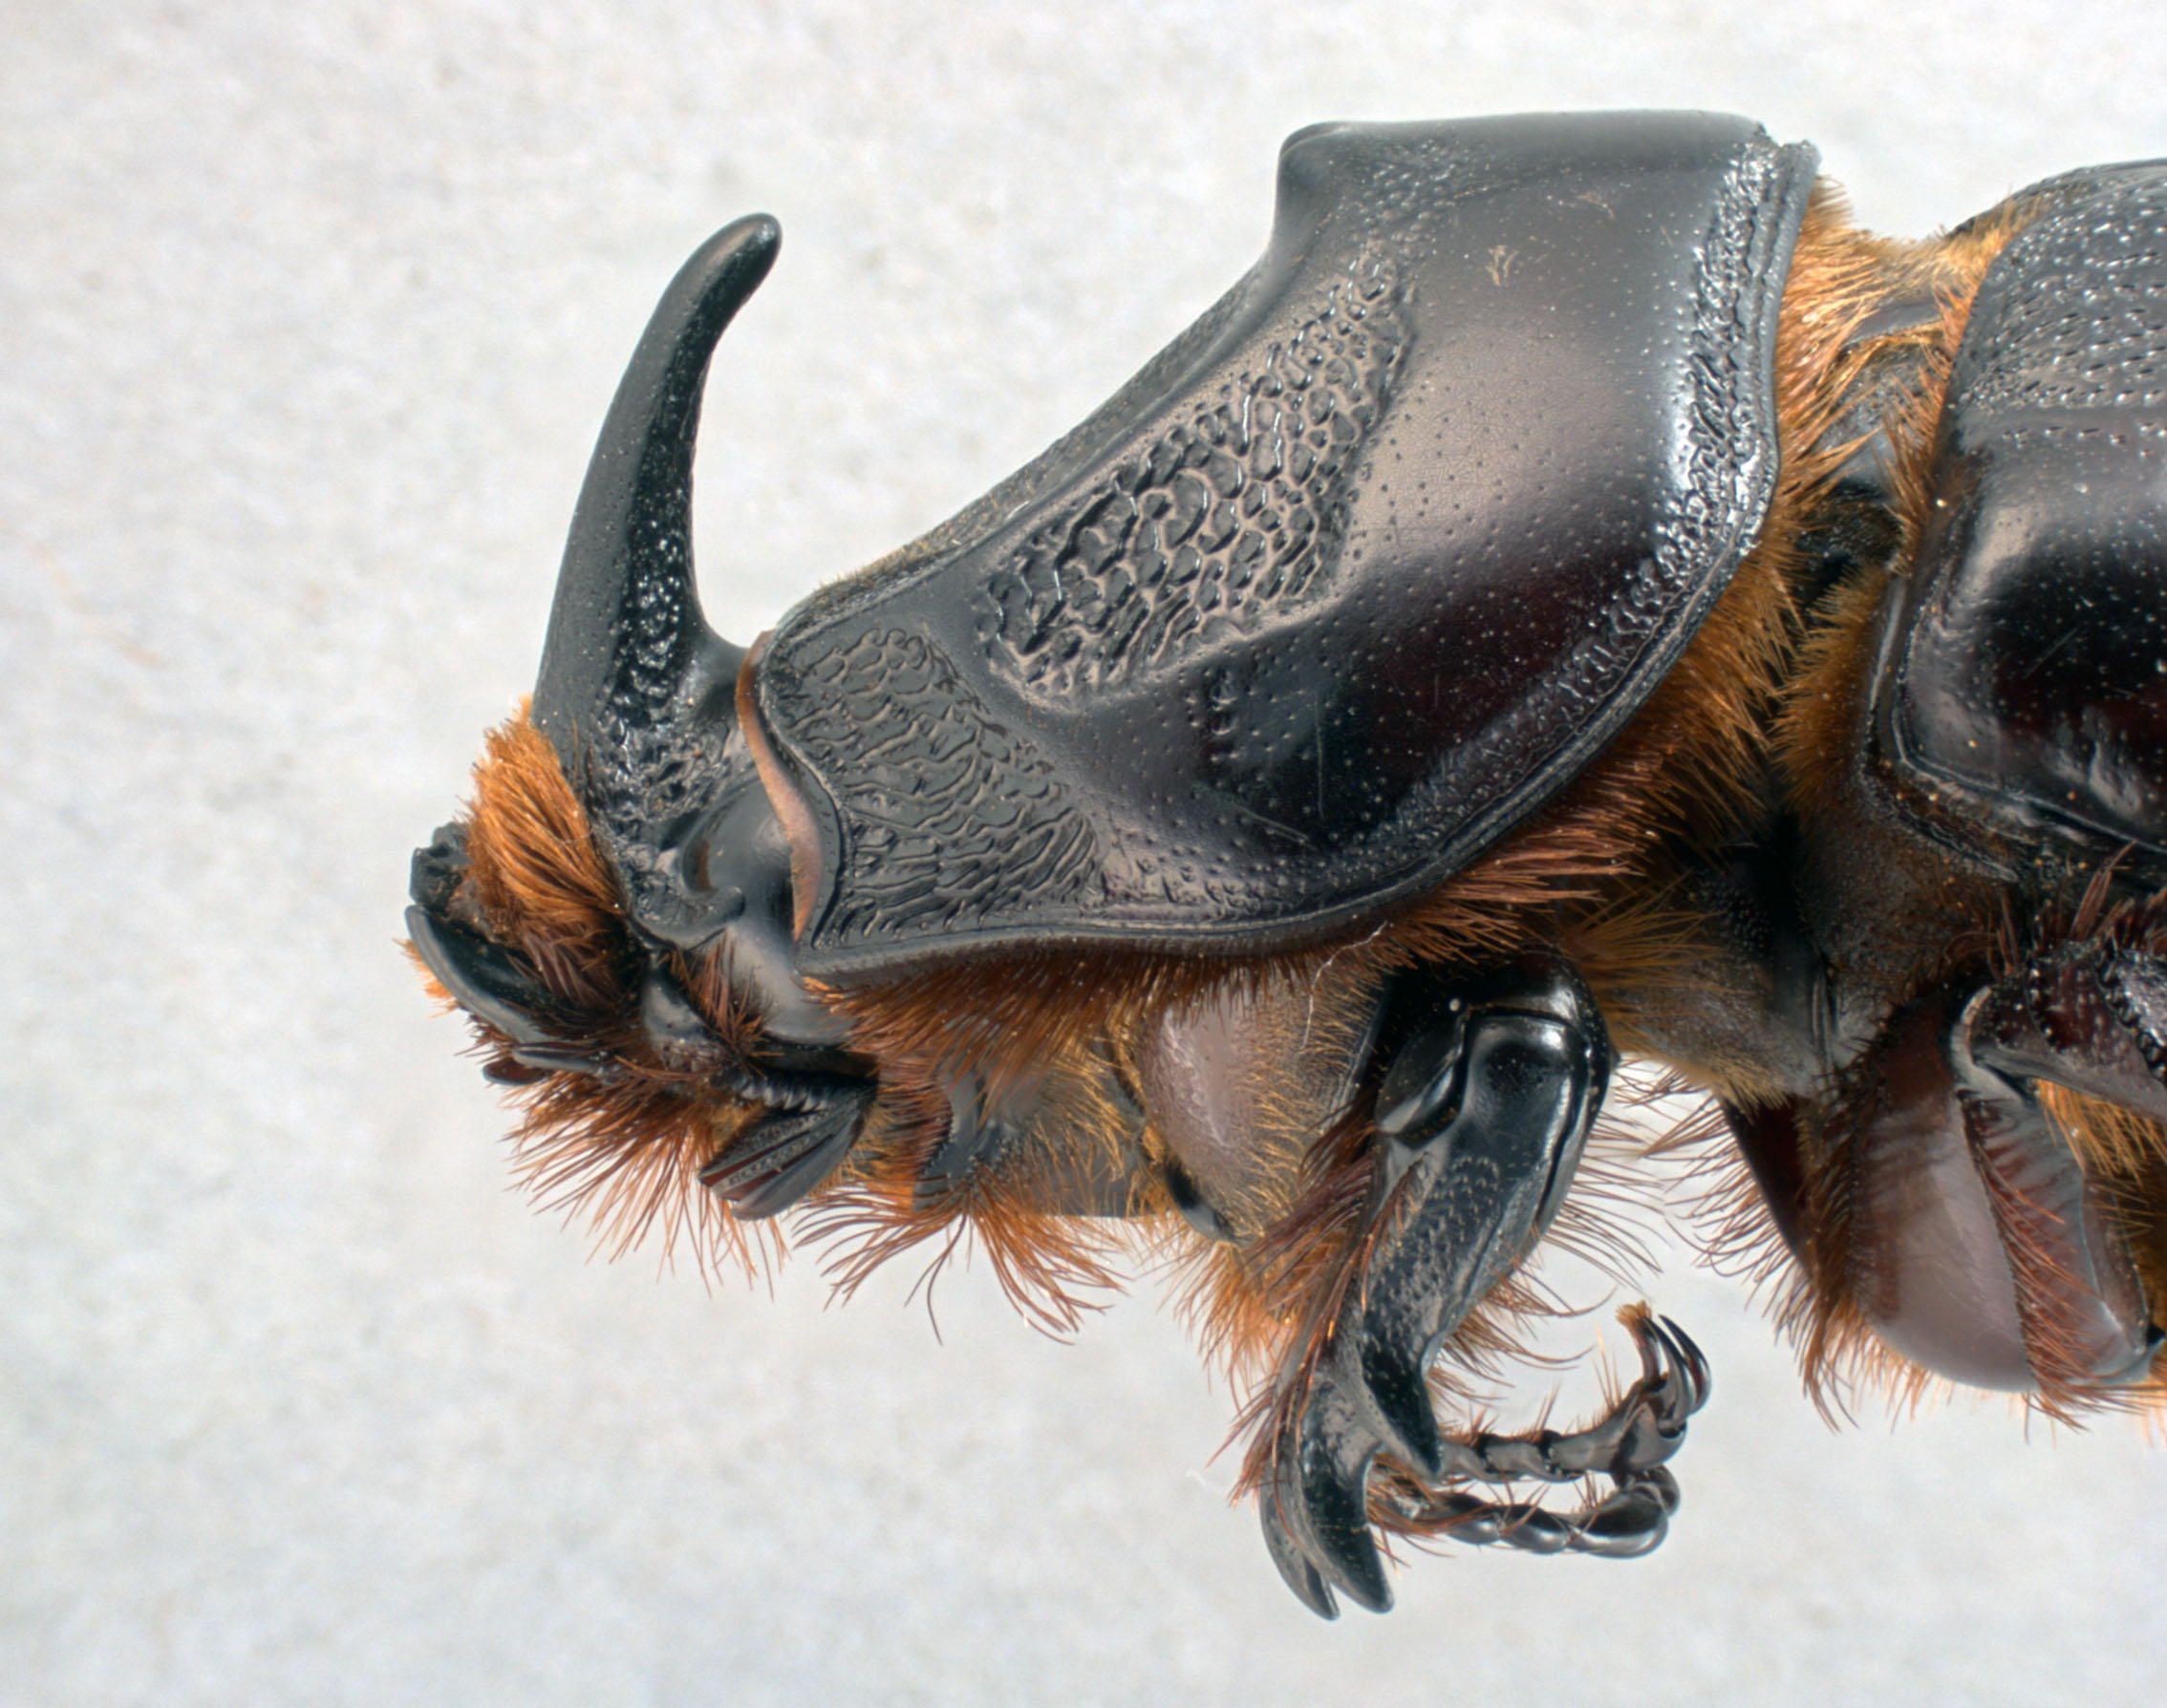
\includegraphics[width=\linewidth]{images/rhino_beetle_head}
	\caption{Male coconut rhinoceros beetle head and pronotum.}
	\label{fig:rhinobeetlehead}
\end{figure}

Coconut rhinoceros beetle (CRB) (Fig. \ref{fig:rhinobeetlehead}), \textit{Oryctes rhinoceros} (L.) (Coleoptera: Scarabaeidae) is a major pest of coconut palm and oil palm. It is native to southeast Asia, but its has invaded many Pacific islands and its range is currently expanding towards the Americas.

\section{Biology}

\subsection{Taxonomy}

The coconut rhinoceros beetle (CRB), \textit{Oryctes rhinoceros} L., is a member of the scarab beetle  family, Scarabaeidae, and the subfamily Dynastinae. Taxonomic expertise is required to differentiate \textit{O. rhinoceros} from serveral other similar \textit{Oryctes} species, some of which also attack coconut and other palms.


\subsection{Life cycle and reproduction}
CRB has four life stages: eggs, grubs, pupae and adults with the grubs having three substages called instars (Fig. \ref{fig:crblifecycle}). The life span depends on environmental conditions, varying between 9 months and 18 months and generation time varies between 5 months and 9 months.
The CRB sex ratio is usually close to 50:50 and females lay about 65 eggs during their lifetime. Under optimal environmental conditions with an unlimited food supply, CRB populations have the potential to grow at a rate of 3,250\% per generation.

\begin{figure}[h!]
	\centering
	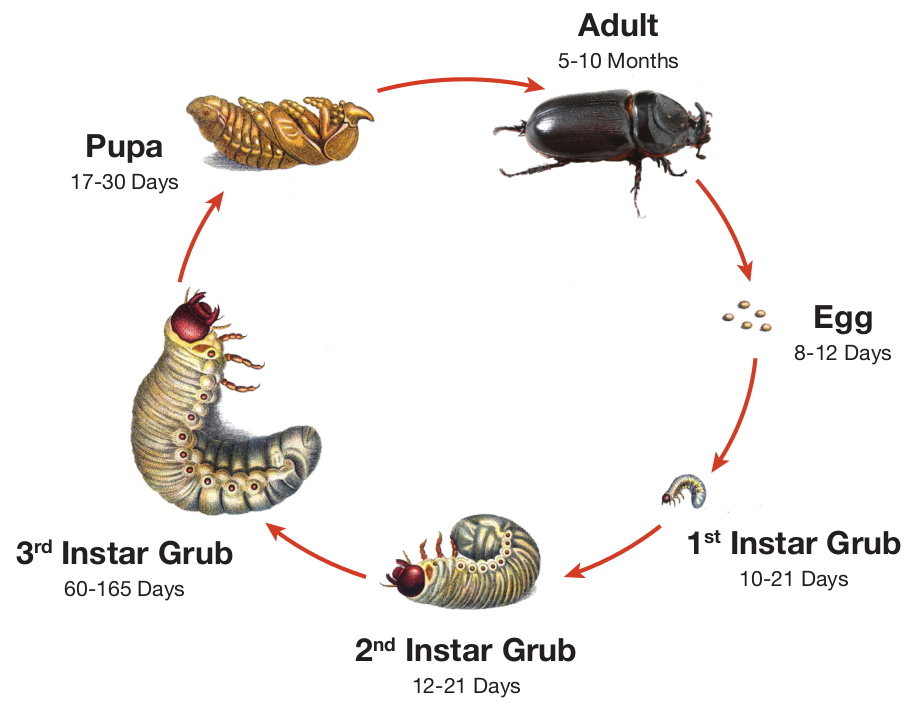
\includegraphics[width=\linewidth]{images/crb_life_cycle}
	\caption{Coconut rhinoceros beetle life cycle.}
	\label{fig:crblifecycle}
\end{figure}

Like all beetles, CRB has four life stages: egg, grub, pupa, and adult (Fig. \ref{fig:crblifecycle}). Only the adult stage causes damage. Grubs feed only on decaying vegetation and do no harm. Adult males and females bore into the crowns of coconut palms and other palms to feed on sap. 

Adults do not feed on leaves, but they bore holes through developing leaves on their way to the white tissue at the interior of the crown. When these damaged leaves eventually emerge from the crown, they have v-shaped cuts in them, a distinctive sign of CRB damage (Fig. \ref{fig:dyingcoconuts}). Each adult feeds on sap for only a few days. It then leaves the crown to search for a breeding site. Palms may be killed if a CRB bores through the growing tip (the meristem). Mature palms are rarely killed at low CRB population levels. However, trees are killed when they are simultaneously attacked by many adults during a population outbreak such as the one we are currently experiencing on Guam. Coconut rhinoceros beetles attain maximum mass at the end of the third instar. Adults are at maximum mass when they have just emerged from the pupa.

All life stages aggregate in CRB breeding sites which can be found wherever vegetation accumulates. Preferred sites are standing dead coconut stems and fallen coconut logs and fronds. But piles of anything with a high concentration of decaying vegetation can be used as a breeding site including green-waste, dead trees of any species, saw dust, and manure. CRB breeding sites have even been found in commercially bagged soil purchased from a local hardware store [3]. 
%An active breeding site will contain all CRB life stages. Adults locate breeding sites by sniffing out a chemical signal referred to as an aggregation pheromone. This pheromone has been synthesized and is commercially available [4].

A female CRB lays about 100 eggs during her lifetime. Assuming a 50\% sex ratio and 100\% survival, there will be a population increase of 5,000\% during each generation. Thus population explosions may occur when abundant potential breeding sites are available in the form of rotting vegetation following destruction in the wake of a typhoon, large scale land clearing, or war. Large numbers of CRB adults generated by a population explosion may result in large numbers of palms being killed. The dead standing trunks soon become ideal breeding sites which generate even higher numbers of adults. This positive feedback loop will end when the rhino beetles run out of food, meaning when most of the palms have been killed and rotted away.

\subsection{Damage caused by CRB}
Grubs feed in almost any type of dead vegetation, including animal manure,  and they do no damage. However, both male and female adults bore into the crowns of palms to feed on sap. Each feeding event lasts only a few days and each adult may feed several times before it dies. Damage is caused when the beetle bores through developing fronds. When these fronds emerge from the crown they exhibit distinctive v-shaped cuts. This damage results in reduced photosynthesis, fruit production and loss of aesthetic quality in ornamental palms. If a bore hole passes through the meristem (growing tip), the palm will not be able to produce new fronds and it will die within about a year when all existing fronds senesce and fall off. Mortality caused by CRB is often seen in young palms but it is rare in mature palms unless there is a high population of CRB adults. 

Some host plant lists for CRB are misleading. Grubs can be found in decaying material from many plant species such as LIST HERE. Accumulation of detritus in coconut palm crowns on Guam. Dead limbs.

Adults will occasionally bore into live plants to feed on sap for a few days. Banana pandanus cycads etc.

\begin{figure}[h]
	\centering
	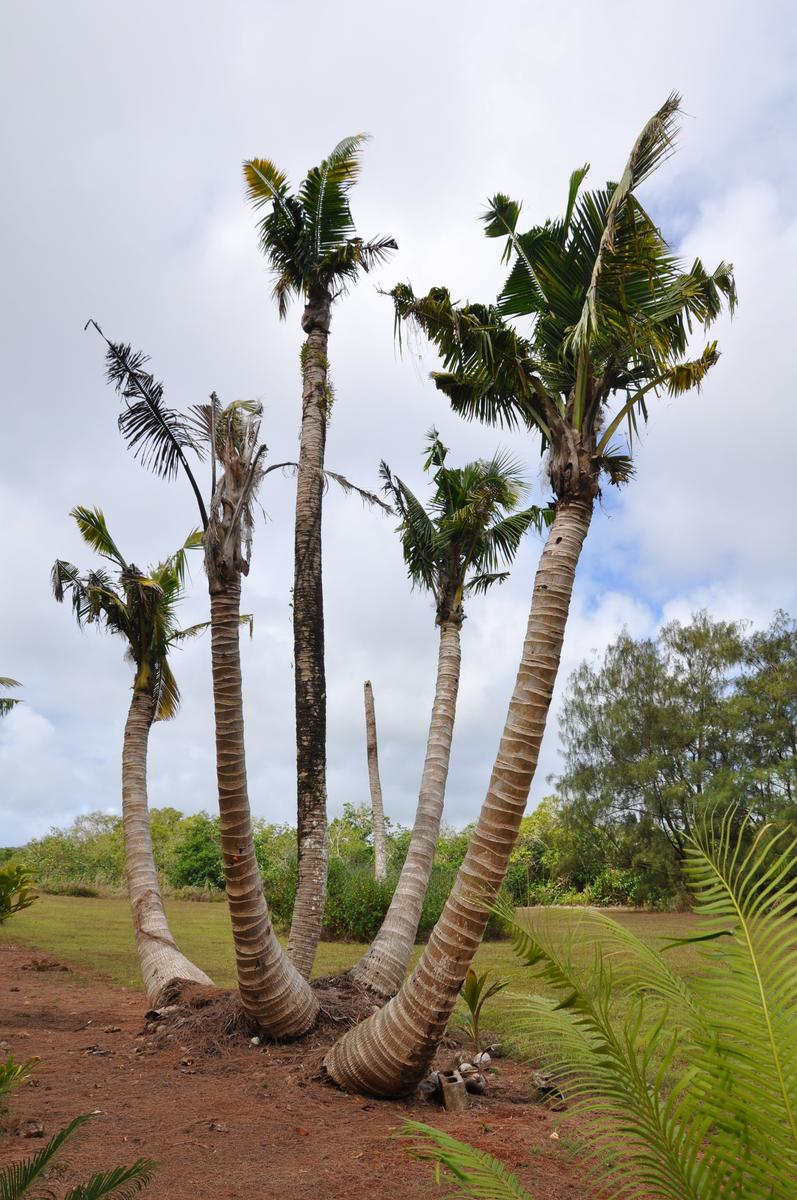
\includegraphics[width=0.8\linewidth]{images/dying_coconuts}
	\caption{Coconut palms severely attacked by coconut rhinoceros beetle.}
	\label{fig:dyingcoconuts}
\end{figure}

\subsection{Population dynamics}
Dead palms quickly become ideal CRB breeding sites. Large numbers of dead palms killed by CRB adults or  large accumulations of dead vegetation caused by tropical cyclones, massive land clearing or military activity may lead to a self-sustaining  CRB outbreak: CRB adults kill palms which become breeding sites. CRB adults emerging from these breeding sites kill surrounding palms, creating new breeding sites which generate even more adults which kill even more palms. An example of this positive feedback cycle occurred in Palau as a result of massive destruction of palms and other vegetation during the Second World War. Prior to the war, CRB was very rare in Palau but shortly afterwards about 50\% of coconut palms were killed by CRB.

\subsection{Geographic distribution}

CRB invaded islands in the Pacific and Indian Oceans during two waves of movement (Fig. \ref{fig:crbdist}). The first wave occurred started in 1909 when CRB was accidentally transported to from Sri Lanka to Samoa with shipment of rubber tree seedlings and it ended during the 1970s
[5]. All of the CRB range expansion during this period was south of the equator except for the invasion of the Ryuku Islands (Japan) starting in 1921 [6] and invasion of the Palau Islands in about 1942 [5]. In Palau, there was a population explosion of rhino beetles because WWII activities created abundant breeding sites. This resulted in about 50\% coconut palm mortality overall, and total loss of coconut palms on some of the smaller islands [7].

\begin{figure}
	\centering
	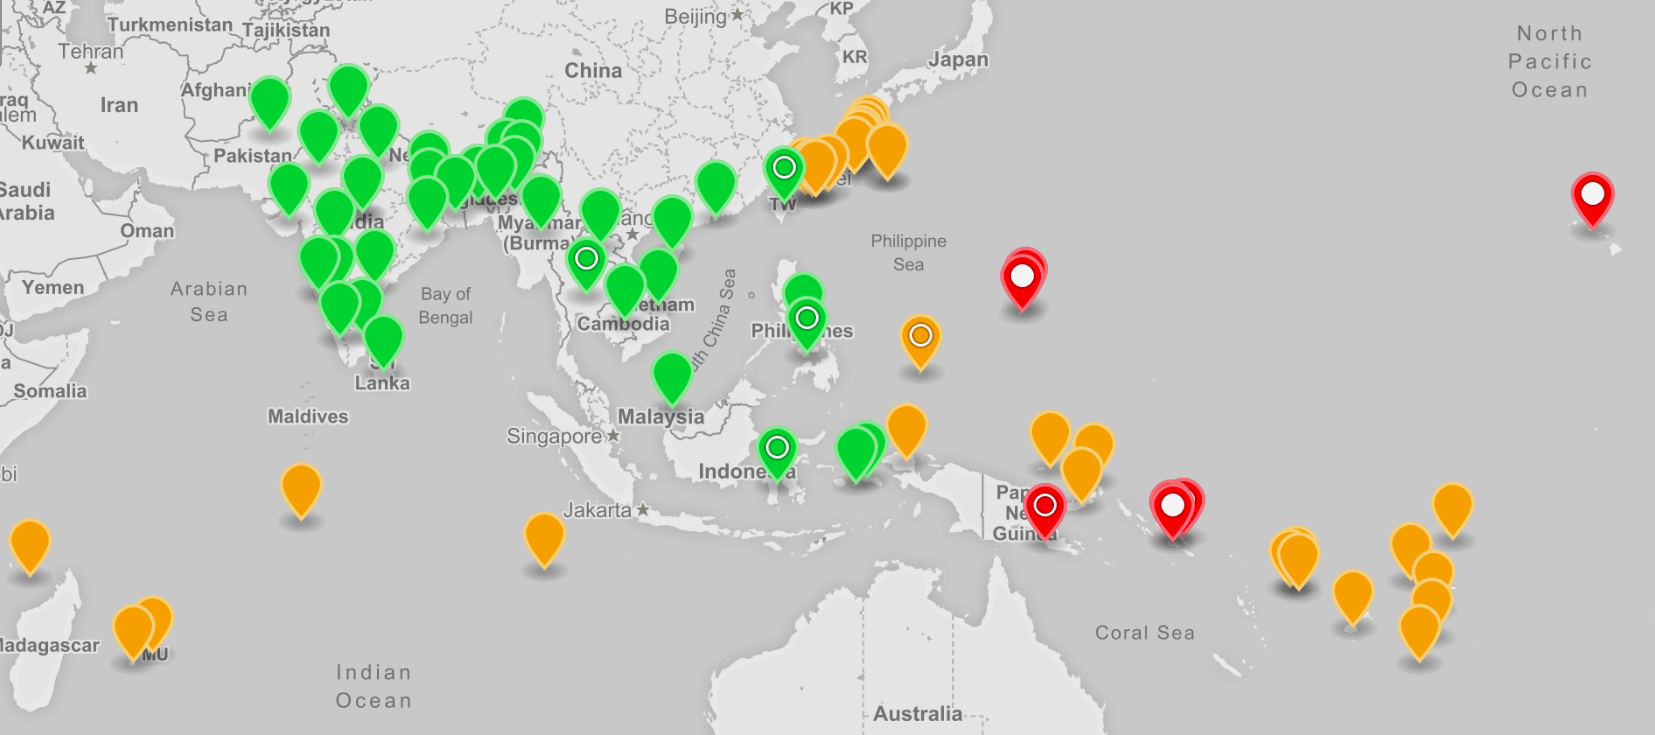
\includegraphics[width=\linewidth]{images/crb_dist}
	\caption{Screenshot of an online interactive web map \cite{moore_web_2019} showing the geographic distribution of the coconut rhinoceros beetle. Green markers: native range; Orange markers: first detected during the 20th century; Red markers first detected during the 21st century; Open circle: population includes CRB-G biotype; Filled circle: population is exclusively CRB-G biotype.}
	\label{fig:crbdist}
\end{figure}

The second wave of CRB invasions started in 2007 with discovery of CRB on Guam, followed by invasion of Oahu (Hawaii), Port Morseby (Papua New Guinea), Guadalcanal, Savo and Malaita (Solomon Islands), and Rota (Commonwealth of the Northern Mariana Islands). Beetles in the second wave of invasions are genetically different from those in the first wave [8] and these are being referred to as the Guam biotype or CRB-G for short.

\section{Control actions for CRB}

\subsection{Eradication}

In theory, eradication of CRB from a newly invaded area can be attained by blocking invasion pathways coupled with finding and destroying all breeding sites. In practice, eradication has proven to be very difficult after initial establishment of a CRB population, despite early detection and rapid response. 

Only one of many eradication attempts has succeeded. This was accomplished on the tiny (36 km\textsuperscript{2}) Niuatoputapu Island (also known as Keppel Island), which lies between Samoa and Tonga. During a period spanning 1922 to 1930 all CRB breeding sites were located and destroyed.


%
%CRB is endemic to Southeast Asia where the distinctive v-shaped notches caused by adult feeding are seen frequently in coconut palms but the damage is seldom sufficient to warrant control. The insect becomes a pest, 
%causing severe damage, where there is an abundance of old palm trunks and organic matter, such as that left after cyclones or after felling senile palms for establishment of new plantations (Figure 3.1). In these conditions,female beetles will fly into the area and lay eggs in the organic matter with high numbers of larvae developing in the decaying material. When this generation emerges, the numbers of beetles and the continuing abundance 
%of food resources can lead to a population explosion and emergence of particularly high numbers in the second generation. These numerous emergent adults will cause significant damage to the nearby palms, even killing 
%many, which leads to further substrate availability and an ongoing problem from the beetles. 

\subsection{Sanitation}

Sanitation includes detection and destruction of active and potential CRB breeding sites.

\paragraph{Breeding site detection}

Local searches for breeding sites are usually initiated in response to visible damage to palms or capture of adults in pheromone traps. In Guam and Hawaii, dogs trained to sniff out CRB grubs have been deployed to assist human searchers. Recent research suggests that CRB adults fitted with miniature radio transmitters or harmonic radar tags may be a cost effective way of detecting cryptic breeding sites. The essential idea is that the radio transmitters and tags will accumulate at breeding sites where adults aggregate. They can then be detected by ground and/or aerial surveys using radio receivers or harmonic radar transceivers.


%is a process to remove organic matter sources and is especially important to prevent establishment of new populations and to limit the damage from established populations. CRB larvae feed and grow in rotting organic  matter.  The  life  cycle  can  be  disrupted  and  populations  reduced  if  bulk  sources  of  organic  matter can be removed, or at least reduced. Sanitation methods are reviewed in Godshen (2015) and the sanitation 
%programme carried out on Guam has been described by Smith and Moore (2008). Where sanitation is part of the response to a recent invasion by CRB, it is important to keep thorough records of clean-up activities. In any programme to control CRB, a sanitation plan should be developed and carried out, as outlined below.

\paragraph{Removal of standing dead palms}
CRB adults are attracted to standing dead palm trees that have begun to rot from the crown. Females will lay their eggs in the rotting palm trunk and the developing larvae will feed on the decaying fibers near the top of the trunk, which starts to decompose in the center forming a protective tube for larval development. As the larvae increase in size and strength of their mandibles, they can penetrate further down the trunk leaving a column of frass and cut fibers for the early instars. Dead standing palms should be felled, cut into pieces and burnt or buried to remove potential breeding sites. In some situations, larvae may develop in the crown of live palms. This only occurs where there are large accumulations of organic matter in the frond bases. The organic matter should be removed where possible.

\paragraph{Disposal of dead felled palms}
Mature palm trees will fall after being weakened by fungal diseases (\textit{Ganoderma}), after strong winds during tropical cyclones or after the felling of senile palms prior to replanting. Dead palms on the ground should be cut up into manageable lengths or chipped prior to disposal by burning or deep burial. 

\paragraph{Covering of palm stumps}
Felled palms leave a stump which is suitable for development of larvae as it rots. In management of palm plantations in Asia, where a zero-burning policy is in operation, ground cover is planted shortly after felling to cover the debris and make it less attractive to the flying beetles. The legumes \textit{Mucuna} spp. and \textit{Pueraria javanica} are ground cover plants that are commonly used, as they will add nitrogen to the soil and cover the decaying trunks. 

\paragraph{Management of organic matter and compost}
Heaps  of  organic  matter,  particularly  palm  debris,  provide  excellent  food  material  for  development  of  CRB larvae. Any deep piles of organic material will be attractive to the egg laying females. Heaps of fronds or empty fruit bunches are particularly susceptible. Sawdust from sawmills that process palm timber is also a favorable resource for beetle development. General compost, farmyard manure and even organic garbage can provide sites for development of the larvae. The first step in reducing the threat of beetles emerging from composts is management of the organic matter. Palm debris should be spread among the palms to break down rapidly and release nutrients rather than being piled in heaps. Compost or farmyard manure should be turned regularly, and larvae removed, or pigs and chickens can assist by eating exposed larvae. In urban environments, organic material is often gathered during environmental clean-up and composted, but this may provide a centre for re-infestation of the locality. Compost can be sterilized or fumigated to kill larvae; however, this process is energy-demanding  and  expensive.  Sterile  compost  will  also  be  susceptible  to  re-invasion. Where  feasible,  compost heaps can be covered with netting to trap emerging beetles.

Burning CRB breeding material is the most dependable method for removing the food source for CRB grubs. In Hawaii CRB sanitation programs, breeding site material is being burned on-site using air-curtain burners and some is being trucked to a waste-to-energy electrical power generation plant. 

\subsection{Trapping}

CRB trapping can be used for different purposes including surveillance for early detection, monitoring growth and spread of a population over time, and for population suppression by mass trapping. In all cases, the trap needs to be attractive enough to draw in beetles from a distance strong and enough to contain them once they are captured. Olfactory and visual attractants can be used to increase trap catch. 

\paragraph{Artificial breeding sites} One of the first traps to be developed was the Hoyt trap made from a metal can set on top of a coconut trunk or wooden post. The can was capped with a length of coconut stem with a hole in the center large enough for a beetle to enter. The trap system was used extensively and functioned because it mimicked a standing, decaying coconut stem which is attractive to CRB adults. Another early trap system was simply a pile of coconut log sections placed on the ground.

FIGURE NEEDED: HOYT TRAP, LOG TRAP, PANEL TRAP

\paragraph{Pheromone traps} Design and utility of traps changed with the discovery of ethyl chrysanthemate as an attractant. This was rapidly superseded by ethyl-4-methyloctanoate (E4-MO) commonly referred to as oryctalure, the male-produced aggregation pheromone of CRB, which could be synthesized. E4-MO attracts both sexes, has been used for more than 30 years and is produced commercially by several companies. 

Pheromone traps for surveillance need to be robust, inexpensive, attractive to beetles, difficult to exit and simple to service. Bucket traps, often with vanes, have been used in surveillance trapping in Guam and Hawaii where thousands of traps have been distributed and monitored for delimitation of the spread of CRB populations and to monitor success of control activities. Bucket traps have also been used extensively for monitoring throughout the Pacific Islands and Southeast Asia. Panel traps?

NEED FIGURE OF BUCKET TRAP (VANED AND UNVANED) AND PANEL TRAP

%Construction of a bucket trap
%
%The pheromone bucket trap can be constructed from a plastic bucket with a lid. Two large holes (with a diameter 
%of 2.8 centimetres) and 2 small holes (in the centre) should be made in the lid as illustrated below. The holes can 
%be cut using a hot wire or hot rod. 
%
%The pheromone sachet should be opened and attached with a wire under the bucket lid. The operator should 
%ensure the sachet is not damaged and that it is placed in an upright position inside the bucket. 
%
%The lid should be placed on the bucket (serving as the pheromone trap). In the field, the pheromone trap 
%should be placed on a strong branch with the bucket hanging upright (Prasad S and Lal S, 2006). For diagnostic 
%purposes, such as DNA analysis, beetles should be removed at least once per week and stored individually 
%in plastic containers. If used for monitoring adult beetle numbers, the bucket should be emptied at three-
%week intervals and the collected beetles destroyed. Pheromone sachets need to be replaced every 6–8 weeks 
%(average), given the tropic heat and evaporation levels.
%
%A more costly alternative to the bucket trap is the pipe trap (Figure 3.2D), which was developed by the oil palm 
%industry in PNG and has been widely used. It is made from a two-metre section of PVC piping secured to an 
%iron bar above a collection tray. Two “windows” are cut into the pipe near the top, which aid entry of the beetles 
%before they fall into the collection chamber. Pipe traps are fixed in surveillance sites and suitable for long-term 
%monitoring. 
%
%Sachets of E4-MO can be placed in either bucket or pipe traps as a lure for the beetles. Traps should be placed 
%in a location that is attractive to the flying beetles (on a ridge or in a specific tree) with the aim of obtaining a 
%consistent representative sample of beetles. The trap position should be fixed (by map or GPS) and recorded. 
%The  traps  should  be  cleared  regularly  (usually  every  7–14  days)  with  beetles  differentiated  into  males  and 
%females and numbers recorded. Sachets of lure should be replaced when they appear to have dried out. This 
%depends on weather conditions, but sachets usually last 1–4 months. 

%The E4-MO pheromone is an aggregation pheromone that is attractive to both male and female beetles. The 
%pheromone assists the general orientation of the beetles. However, they are not able to identify the precise 
%location and many will arrive in the vicinity of the trap without entering it. This can result in higher damage to 
%palms close to the trap when compared with the average of the whole plantation.
%
%In the office, trap catches should be analysed, preferably mapped and summarised. The trap catch should be 
%converted to beetles trapped per day, as this figure will be comparable between sites and dates for the same 
%type of trap. An example is presented below, with daily trap catch mapped with time (Figure 3.3). 
%
%Trap information should be complemented with regular photographic assessment of palms around the sample 
%area and satellite images may be used to assist monitoring. Dated satellite images from Google Earth PRO can 
%also be used to provide an indication of changes in damage over time.

\paragraph{Efficacy of pheromone traps for population suppression} Trapping will remove insects from the population and can contribute to pest and damage reduction. Bucket traps baited with pheromone have been reported to reduce CRB populations in Malaysia and the related \textit{O. monoceros} in West Africa. 

It has been suggested that mass trapping can eradicated newly detected population of CRB by trapping all adults, thus preventing all reproduction and damage. Mass trapping was performed on Guam shortly after detection of CRB in the Tumon Bay hotel are in 2007. These traps did not mitigate damage to palms with the mass trapping areas. During 2010, the trap catch rate in Tumon Bay was only 0.006 beetles per trap day, but CRB damage was visible in 100\% of coconut palms. In contrast, a similar mass trapping program in Samoa trapped 0.150 per trap-day, but the proportion of damaged coconut palms was 30\%. Note that the Guam population is the CRB-G biotype and the Samoan population is the CRB-S biotype. Three possible explanations have been suggested to account for these observations:
\begin{enumerate}
	\item Traps baited with oryctalure are more attractive to CRB-S than CRB-G.
	\item CRB-G individuals do far more damage than CRB-S individuals.
	\item At very high population levels and trap densities there is so much pheromone in the air that beetles cannot navigate to pheromone sources
\end{enumerate} 


but had very little effectcan be eradicated  However, bucket and pipe traps are not 
sufficient for high-density, invasive populations. 

Improving trap efficiency has been a goal of the research team at the University of Guam where a range of 
innovative trap designs have been developed (Moore et al. 2014; Iriate et al. 2015). Bucket trap catches have 
been improved by expanding the size (a barrel trap), and adding organic matter to the trap and a small LED 
light. 

Following a suggestion that 

\paragraph{Tekken fish net traps} In an alternative approach, fish nets made from Tekken netting have been used (Figure 3.4). These act like 
a fishing gill net, catching beetles as they try to move through it. In Guam, covering heaps of organic waste with 
Tekken netting has been successful as it catches fresh adults as they emerge from organic waste, where they 
have developed, as well as beetles that are returning to the organic matter heaps to lay eggs. Netting can also 
be used in simple traps baited with pheromone on fences or by looping around the palm trunk to entangle the 
adult beetles as they move to the palm (Moore et al. 2014).

\begin{figure}[h]
	\centering
	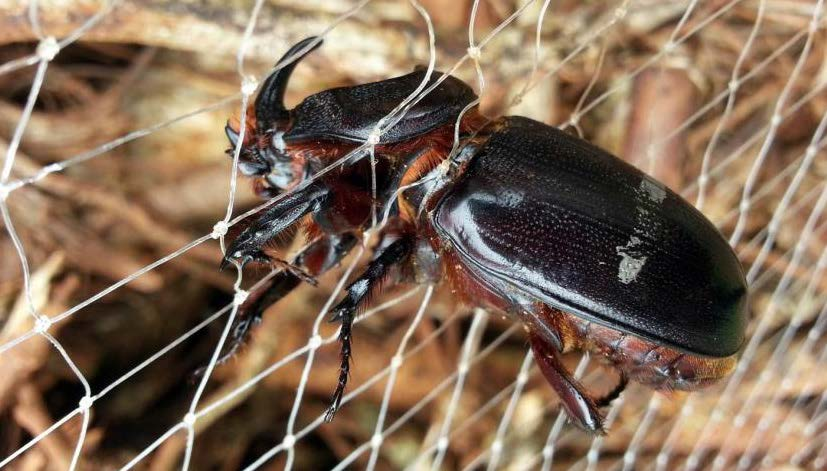
\includegraphics[width=\linewidth]{images/tekken-beetle}
	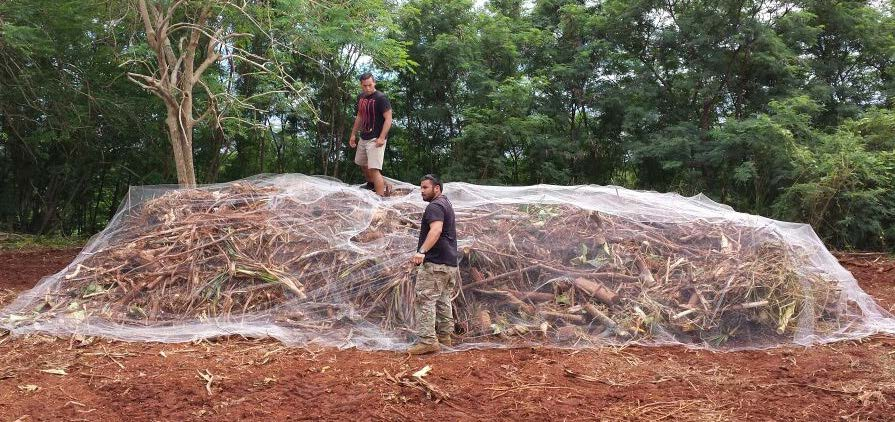
\includegraphics[width=\linewidth]{images/tekken-pile}
	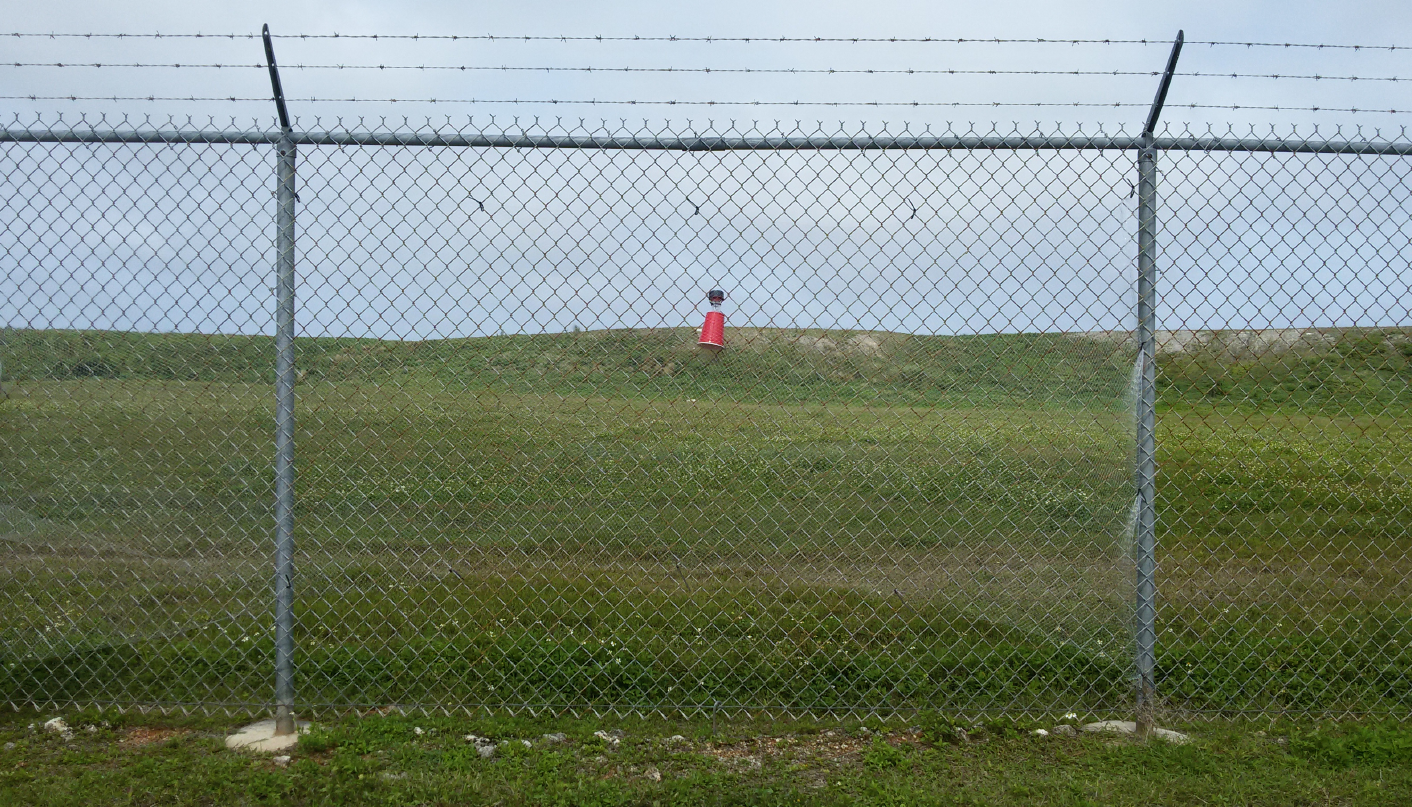
\includegraphics[width=\linewidth]{images/defence-trap}
	\caption{Tekken.}
	\label{fig:tekken-beetle}
\end{figure}

Trapping has been used successfully for both monitoring and control. The Hoyt trap was used to monitor the 
decline of beetle numbers over three years, which was associated with a loss of organic matter for larval feeding 
(Bedford 1975). Pheromone traps baited with E4-MO can be placed at one trap per 10 hectares to monitor 
populations in order to establish control action thresholds, or they can be placed at high densities, one per two 
hectares, in order to reduce CRB populations in plantations (Chung 1997). With improvements in trap design, 
Moore et al. (2014) estimated the capture of 33 per cent of a CRB population, which would have a significant 
impact on the population especially if combined with other measures. Tekken netting tied around the palm 
through  the  leaf  axils  seems  particularly  effective  in  protecting  young  ornamental  palms  from  attack  as  it 
intercepts the beetles as they move towards the feeding site. 

%\subsection{Mechanical control}
%CRB adults in freshly damaged palms can be located and killed by workers using a wire hook in a process known 
%as winkling. As the beetle bores into the palm petiole (Section 2.5), it produces an excessive amount of cut 
%fibrous material as it drills into the trunk (Fig. 2.8). This will be evident in the axils of the fronds and will indicate 
%the presence of a beetle. A wire can be inserted into the hole and, with skill, the beetle can be removed from 
%the hole and killed. Winkling is mostly used in oil palm where most damage occurs in the crown of young palms 
%and the fresh fibres produced by the beetle can be easily seen. Winkling in coconut palms is more difficult as 
%the worker must climb the palm to see the damage. 

\subsection{Chemical control}
Chemical  control  measures  are  most  effective  on  young  palms  against  CRB.  Chemical  pesticides  are  used to  prevent  the  adult  beetle  from  damaging  the  spear  and  growing  point.  The  insecticide,  cypermethrin,  is recommended to protect young oil palm replants in CRB-infested areas but only until the palm starts fruiting as the insecticides can damage the beneficial pollinating weevil (Elaeidobius kamerunicus) (Ismael et al. 2009). 
Moore (2013) also tested use of cypermethrin for control of CRB in coconut palms in Guam and found it effective when applied to young damaged palms. Trunk injection with Thiosultap disodium (Ero 2016) has also been shown to kill beetles in the crown of mature oil palms (Ero pers. comm.). Some insecticide options for CRB have been described by CABI (www.cabi.org/isc/datasheet/37974); however, their use is limited given the intermittent pattern of attack and the growth of the palms making the crowns unreachable. As the target for protection is the base of the frond sheath where the beetle penetrates the petiole, granular formulations are an option to facilitate application. Use of any insecticide should conform to the registration regulations of the country of use and be applied with appropriate care. Guidelines for application of synthetic pesticides are provided in SPC documents (e.g. Crop Protection Manual for Trainees, Honiara, Solomon Islands 2012).

\subsection{Biological control}

Biological control is the use of natural enemies (predators, pathogens, parasites) to suppress pest populations 
(Van Driesche and Bellows 1996). In its native range, CRB is attacked by a community of co-evolved natural 
enemies (reviewed by Bedford 1980), including pathogenic viruses and fungi, predatory carabid and elaterid 
beetles  and  parasitic  Scolia  wasps.  The  relative  impact  of  each  natural  enemy  species  within  this  native 
community is poorly known, with additional control strategies often needed to complement biological control 
in coconut and oil palm plantations. (See IPM section 3.6.)

When  CRB-S  invaded  the  Pacific,  it  was  the  focus  for  a  substantial  biological  control  programme.  The  aim 
was to find one (or more) natural enemies in the native range that could be introduced to the invaded range 
to  suppress  CRB-S  populations  (e.g.  Hoyt  1963).  This  process  is  known  as  classical  biological  control  (Van 
Driesche and Bellows 1996). Among many natural enemies introduced to the Pacific, very few predators or 
parasites established (Caltagirone 1981). Incidental predation by pigs and chickens on CRB larvae may assist 
with control of this pest and can be useful for control of larvae in household or community waste piles. Local 
species of generalist arthropod predators (centipedes, beetles, ants) may feed on CRB larvae; however, there is 
little evidence that this contributes significantly to CRB control (Hinckley 1967). Only one pathogen provided 
significant control of CRB-S: the Oryctes rhinoceros nudivirus (OrNV) discovered in Malaysia by Alois M. Huger. 
(Huger 2005 summarises the history of virus discovery and its use against CRB.) This virus infects CRB larvae and 
adults, causing death after 6–30 days. Infected adults are weakened prior to death so that they stop feeding, 
and their mobility and breeding is reduced. Once established in countries invaded by CRB-S, the virus had a 
significant impact on CRB populations and reduced palm damage (Huger 2005). Another approach to biological 
control for CRB was to create a biopesticide from a known pathogen. CRB adults and larvae can be infected by 
strains of the fungus Metarhizium majus (formerly M. anisopliae var. majus). This fungus has been developed into 
a biopesticide that can be applied to CRB breeding sites in both the native and invaded range (Bedford 2013). 

The recent invasion of CRB-G has changed CRB management wherever it is found. CRB-G is not susceptible to 
the strain of OrNV introduced originally to control CRB-S in the Pacific (Marshall et al. 2017). A new biological 
control effort is underway in order to identify strains of OrNV from CRB’s native range that are effective against 
CRB-G. Until an effective OrNV strain is discovered, biopesticides containing M. majus are the only option for 
biological control of CRB-G. 

\subsection{Integrated pest management (IPM)}

Integrated pest management (IPM), is a broad-based approach that integrates practices for economic control 
of  pests.  The  FAO  defines  IPM  as  “the  careful  consideration  of  all  available  pest  control  techniques  and 
subsequent integration of appropriate measures that discourage the development of pest populations and 
keep pesticides and other interventions to levels that are economically justified and reduce or minimise risks 
to human health and the environment. IPM emphasises the growth of a healthy crop with the least possible 
disruption to agro-ecosystems and encourages natural pest control mechanisms”.

SPC has recommended IPM for management of CRB and includes combination of the factors described above. 

For coconut palms planted for subsistence, ornamental purposes, or in commercial plantations, IPM for CRB 
involves: i) monitoring of palm damage (section 2.5) to detect localised CRB outbreaks and check that control is 
successful; ii) biological control (section 3.5) with OrNV (in the invaded and native range) and other co-evolved 
natural enemies (in the native range only); and iii) sanitation (section 3.1) to remove organic waste, dead palms 
and  other  potential  breeding  sites.  Sanitation  is  an  essential  component  of  IPM  for  CRB  that  complements 

Coconut rhinoceros beetle (Oryctes rhinoceros): A manual for control and management of the pest in Pacific Island countries and territoriesbiological control (Huger 2005). Localised CRB outbreaks will occur when breeding sites are left uncontrolled 
(e.g. after cyclones and tropical storms, when palms are often toppled by high winds and large amounts of 
green waste is created). Historically, outbreaks of CRB often follow cyclone damage (Jackson and Marshall 2017). 
A high number of breeding sites are created during plantation renovation, when old palms are felled to make 
space for replanting. Larvae will develop in the decaying fronds, the trunk and even the root of the felled palm. 
Some additional options may be incorporated into IPM programmes for coconut, particularly for commercial 
plantations or ornamental palms. These more costly options include pheromone traps to monitor adult beetle 
activity and complement it with visual surveys of palm damage. Occasionally, trap catches may be high enough 
to  contribute  to  population  suppression  in  coconut  plantations  (Bedford  2013),  but  this  strategy  is  more 
relevant to oil palm (discussed below). Commercial products containing the fungus M. majus may be applied 
to CRB breeding sites that cannot be removed. Insecticide treatments are not recommended for established 
coconut palms (section 3.4) as there is a potential risk of translocation of insecticides (move within the palm), 
leaving harmful residues in the coconut. If a recent invasion of CRB is targeted for eradication, insecticides 
may  be  necessary  for  success  (Figure  3.6).  In  this  situation,  expert  advice  is  needed  to  determine  the  most 
appropriate choice of insecticide, to advise on the length of time residues will persist, and to ensure insecticide-
contaminated coconuts are not harvested for human consumption. 

For higher value crops, particularly oil palm, the same components are needed as for coconut: monitoring; 
biological control; and sanitation. More costly IPM components are recommended for oil palm because the 
crop’s financial value makes greater investment in control worthwhile (reviewed by Bedford 2014). Thus, IPM for 
CRB in oil palm involves: i) monitoring of beetle activity with pheromone traps (section 3.2) and palm damage 
(section 2.5), particularly for young palms; ii) biological control (section 3.5) with OrNV (invaded and native 
range) and other natural enemies (native range) plus application of M. majus biopesticides to breeding sites 
that cannot be removed; and iii) sanitation to remove organic waste (section 3.1), particularly during plantation 
renewal when large amounts of waste is generated; iv) insecticide treatments (section 3.4) for young palms that 
are most sensitive to CRB damage. Note that pollinators of oil palm are vulnerable to insecticides, so applications 
should be scheduled carefully to avoid flowering. When oil palm plantations are renewed, complete clean-up 
of the organic waste is challenging. In CRB’s native range, an additional strategy is to break up and spread the 
waste as a thin layer, then plant a fast-growing cover crop, often a legume, over the waste matter (Wood 1968). 

A decision tree to identify IPM options for coconut and oil palms is presented below (Figure 3.5). This includes 
decision  points  to  consider  potential  for  eradication  of  recent  CRB  invasions  as  well  as  management  of 
established CRB populations. 

Figure 3.5   IPM decision tree for CRB control in its invasive range. This tree can be used for either CRB-S  
or CRB-G; however, note that an effective strain of Oryctes virus has not yet been identified for CRB-G. 

\newpage
\section*{References}

\paragraph{Bedford, Geoffrey O. 1980.} Biology, ecology, and control of palm rhinoceros beetles. Annual Review of Entomology 25 (1980): 309–39.
Available online at 

\paragraph{Gressitt, J. Linsley 1953.} The coconut rhinoceros beetle (\textit{Oryctes rhinoceros}) with particular reference to the Palau Islands. Bernice P. Bishop Museum. Bulletin 212. 
Available online at

\paragraph{Jackson, Trevor, Sean Marshall, Sarah Mansfield and Fereti Atumurirava 2020.} Coconut rhinoceros beetle (\textit{Oryctes rhinoceros}): A manual for control and management of the pest in Pacific Island countries and territories. Pacific Community (SPC). 
Available online at \url{https://tinyurl.com/yxk4u27j} 

\paragraph{Marshall, Sean D. G., Aubrey Moore, Maclean Vaqalo, Alasdair Noble, and Trevor A. Jackson 2017.} A new haplotype of the coconut rhinoceros beetle, \textit{Oryctes rhinoceros}, has escaped biological control by \textit{Oryctes rhinoceros} nudivirus and is invading Pacific Islands. Journal of Invertebrate Pathology, 149, 127-134.
Available online at 

\paragraph{Pallipparambil, Godshen R. 2015.} New Pest Response Guidelines: \textit{Oryctes rhinoceros} (L.) Coleoptera: Scarabaeidae, Coconut rhinoceros beetle. U.S. Department of Agriculture, Animal Plant Health Inspection Service, Plant Protection and Quarantine.
Available online at \url{https://tinyurl.com/mpdmvfpt}

%\nocite{jackson_coconut_2020}
%
%
%\printbibliography

\end{document}
